\chapter{Mathematical model}

\begin{figure}[h!]
    \centering
    \includegraphics[width=\textwidth]{img/Simulink_transfer.pdf}
    \caption{Block diagram}
    \label{fig:spolerigg3}
\end{figure}

\section{Transfer function for coil rig}

The schematic shown in \cref{fig:spolerigg1} is the schematic for the coil rig. R1 is the resistance in the primary circuit (mainly the cable from the driver to the coil rig), R2 is the resistance in the secondary circuit (mainly the resistance in L2). C1 is the primary capacitor, L1 is the primary coil, L2 is the secondary coil, and C2 is the secondary capacitance (or top load). G1 is the electrical arc modelled as a conductance, see \cref{eq:g1} for the model of G1, this model is a combination of Cassie \citep{cassie} and Mayr \citep{mayr} models for electrical arcs presented in \citep{575670}. $U_p$ is the voltage output from the driver to the primary resonant circuit, $U_s$ is the voltage output from the secondary resonant circuit (the voltage driving the electrical arc).

\begin{figure}[h!]
    \centering
    \includegraphics[width=\textwidth]{Skjema/Spolerigg1.pdf}
    \caption{Caption}
    \label{fig:spolerigg1}
\end{figure}

This schematic can be simplified by introducing the mutual inductance M as a component as shown in \cref{fig:spolerigg2}, and then further simplified by representing the branches of the circuit as impedances as shown in \cref{fig:spolerigg3}.

\begin{figure}[h!]
    \centering
    \includegraphics[width=\textwidth]{Skjema/Spolerigg2.pdf}
    \caption{Caption}
    \label{fig:spolerigg2}
\end{figure}

\begin{figure}[h!]
    \centering
    \includegraphics[width=\textwidth]{Skjema/Spolerigg3.pdf}
    \caption{Caption}
    \label{fig:spolerigg3}
\end{figure}

Using the mesh current method we get \cref{eq:1} and \cref{eq:2}, we then solve these two equations for $I_1$. Set \cref{eq:1_2} equal to \cref{eq:2_2}, solve for $\frac{U_s}{U_p}$ and substitute in \cref{eq:3}. We then have the transfer function $H(s)$ for the coil rig.

\begin{equation} \label{eq:1}
    U_p - I_1 Z_1 - (I_1 - I_2) Z_2 = 0
\end{equation}

\begin{equation} \label{eq:2}
    (I_2 - I_1) Z_2 - I_2 Z_3 - I_2 Z_4 = 0
\end{equation}

\begin{equation} \label{eq:3}
    U_s = I_2 Z_4
\end{equation}

Solve \cref{eq:1} for $I_1$
\begin{equation} \label{eq:1_2}
    I_1 = \frac{U_p + I_2 Z_2}{Z_1 + Z_2}
\end{equation}'

Solve \cref{eq:2} for $I_1$
\begin{equation} \label{eq:2_2}
    I_1 = \frac{(Z_2 - Z_3 - Z_4) I_2}{Z_2}
\end{equation}

Set \cref{eq:1_2} equal to \cref{eq:2_2}, solve for $\frac{U_s}{U_p}$ and substitute in \cref{eq:3}

\begin{equation} \label{eq:3}
    \frac{U_s}{U_p} = H(s) = \frac{Z_2 \cdot Z_4}{Z_1 \cdot (Z_2 - Z_3 - Z_4) - Z_2 \cdot (Z_3 + Z_4))}
\end{equation}

\begin{equation} \label{eq:3_1}
    Z_1 = R_1 + \frac{1}{s C_1} + s L_1 - s M
\end{equation}

\begin{equation} \label{eq:3_2}
    Z_2 = s M
\end{equation}

\begin{equation} \label{eq:3_3}
    Z_3 = s L_2 - s M + R_2
\end{equation}

\begin{equation} \label{eq:3_4}
    Z_4 = \frac{1}{s C_2} + \frac{1}{G_1}
\end{equation}

\begin{equation} \label{eq:3_5}
    M = k \sqrt{L_1 L_2}
\end{equation}

%\begin{equation}
%    H(s) = \frac{s M (\frac{1}{s C_2} + \frac{1}{G_1})}{(R_1 + \frac{1}{s C_1} + s L_1 - s M) \cdot (s M - (s L_2 - s M + R_2) - (\frac{1}{s C_2} + \frac{1}{G_1})) - s M \cdot ((s L_2 - s M + R_2) + (\frac{1}{s C_2} + \frac{1}{G_1})))}
%\end{equation}

% (Z2*Z4)/(Z1*(Z2-Z3-Z4)-Z2*(Z3+Z4)), Z1=(R1+1/(s*C1)+s*L1-s*M), Z2=(s*M, Z3=(s*L2)-(s*M)+R2), Z4=(1/(s*C2))+(1/G1))
Then we have the transfer function of the resonant circuit (shown in \cref{eq:3} through \cref{eq:3_5}), however to be able to analyze this transfer function we have to order it into standard form. Meaning isolating $s$,$s^2$,$s^3$ etc. and expanding the factors. This leads to \cref{eq:4} through \cref{eq:4_4}.

%\begin{equation}
%    H(s) = \frac{s^2 M C_1}{s^4(2 M L_1 C_2 C_1 - L_1 L_2 C_2 C_1) + s^3(2 M R_1 C_2 C_1 - L_2 R_1 C_2 C_1 + 2 M L_1 G_1 C_1 - L_1 R_2 C_2 C_1) + s^2(2 M R_1 G_1 C_1 - R_1 R_2 C_2 C_1 + 2 M C_2 - C_2 L_2 - L_1 R_2 G_1 C_1 - L_1 C_1 + 2 M C_1) + s(2 M G_1 - R_1 R_2 G_1 C_1 - R_1 C_1 - L_2 G_1) - R_2 G_1- 1}
%\end{equation}

\newpage

\begin{equation} \label{eq:4}
    H(s) = \frac{s^3 f + s^2 g}{s^4 a + s^3 b + s^2 c + s d + e}
\end{equation}

\begin{equation} \label{eq:4_1}
    a = (C_1 C_2 G_1 L_1 L_2)-2 (C_1 C_2 G_1 L_1 M)+(C_1 C_2 G_1 M^2)
\end{equation}

\begin{equation} \label{eq:4_2}
    b = (C_1 C_2 G_1 L_1 R_2)+(C_1 C_2 G_1 L_2 R_1)-2 (C_1 C_2 G_1 M R_1)+(C_1 C_2 L_1)
\end{equation}

\begin{equation} \label{eq:4_3}
    c = (C_1 C_2 G_1 R_1 R_2)+(C_1 C_2 R_1)+(C_1 G_1 L_1)+(C_2 G_1 L_2)-2 (C_2 G_1 M)
\end{equation}

\begin{equation} \label{eq:4_4}
    d = (C_1 G_1 R_1)+(C_2 G_1 R_2)+C_2
\end{equation}

\begin{equation} \label{eq:4_5}
    e = G_1
\end{equation}

\begin{equation} \label{eq:4_6}
    f = C_1 C_2 M
\end{equation}

\begin{equation} \label{eq:4_7}
    g = C_1 G_1 M
\end{equation}

Sizes for the parameters in the transfer function is shown in \cref{tab:mod_params} these sizes are rounded approximate sizes for a DRSSTC.

\begin{table}[]
    \centering
    \begin{tabular}{c|c|c|c}
         & Comment &  &\\ \hline
        C1 & Primary load capacitor                 & $10^{-7}$ & F \\
        C2 & Secondary load capacitor (top load)    & $10^{-11}$& F \\
        L1 & Primary coil                           & $10^{-5}$ & H \\
        L2 & Secondary coil                         & $10^{-1}$ & H \\
        M  & Mutual inductance                      & $10^{-3}$ & H \\
        R1 & Primary circuit ohmic resistance       & $10^{1}$  & $\Omega$ \\
        R2 & Secondary circuit ohmic resistance     & $10^{2}$  & $\Omega$ \\
        G1 & Resistance of elecrical arc            & $10^{2}$  & $\Omega$ \\ % Usikker!
        k  & Coupling factor                        & $10^{-1}$ & 
    \end{tabular}
    \caption{Model parameter sizes}
    \label{tab:mod_params}
\end{table}

\todo{Forklare hvorfor disse størrelsene}

\newpage
\subsection{Transfer function for feedback}
If we use \cref{eq:1} and \cref{eq:2} and solve for $\frac{I_1}{U_p}$ we get the transfer function for the feedback signal.
\begin{equation} \label{eq:fb}
\frac{I_1}{U_p} = H_{FB}(s) = \frac{Z_2-Z_3-Z_4}{(Z_1+Z_2)(Z_2-Z_3-Z_4)-Z_2^2}
\end{equation}


\newpage
\subsection{Plots}

Shown in \cref{fig:bode} is the bode plot of the transfer function of the resonant circuit.

\begin{figure}[h]
    \centering
    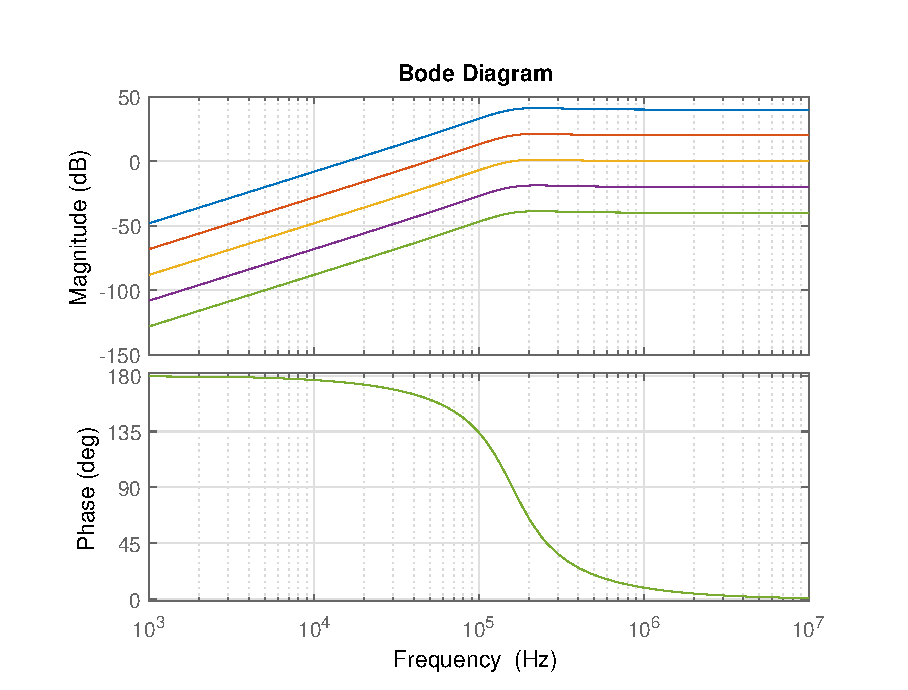
\includegraphics[width=\textwidth]{img/CoilRigBode_M.eps}
    \caption{Bode plot for different values of M}
    \label{fig:bode}
\end{figure}
M is in the range 1e-3 to 1e-7.

\begin{figure}
    \centering
    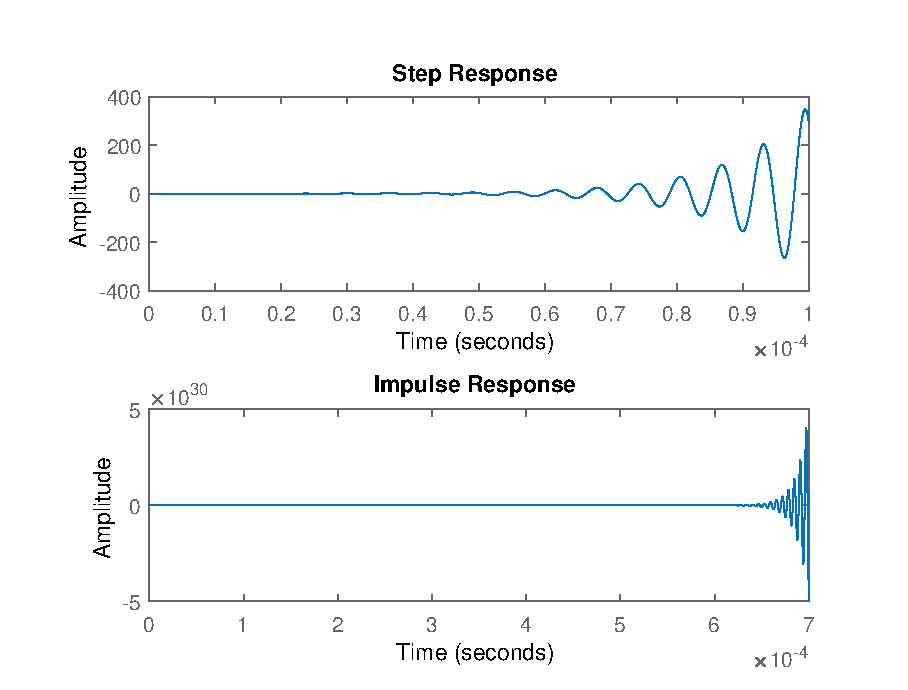
\includegraphics[width=\textwidth]{img/CoilRigResponse.eps}
    \caption{Step and impulse response for M=1e-6}
    \label{fig:my_label}
\end{figure}

\begin{figure}
    \centering
    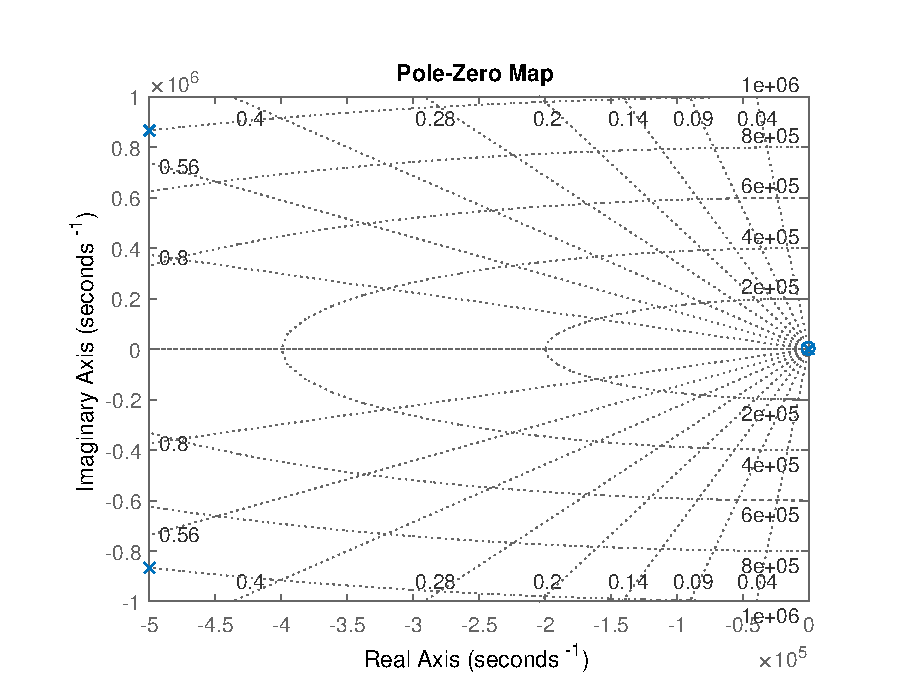
\includegraphics[width=\textwidth]{img/PoleZeroPlot.eps}
    \caption{PoleZeroPlot for M=1e-6}
    \label{fig:my_label}
\end{figure}


\begin{figure}
    \centering
    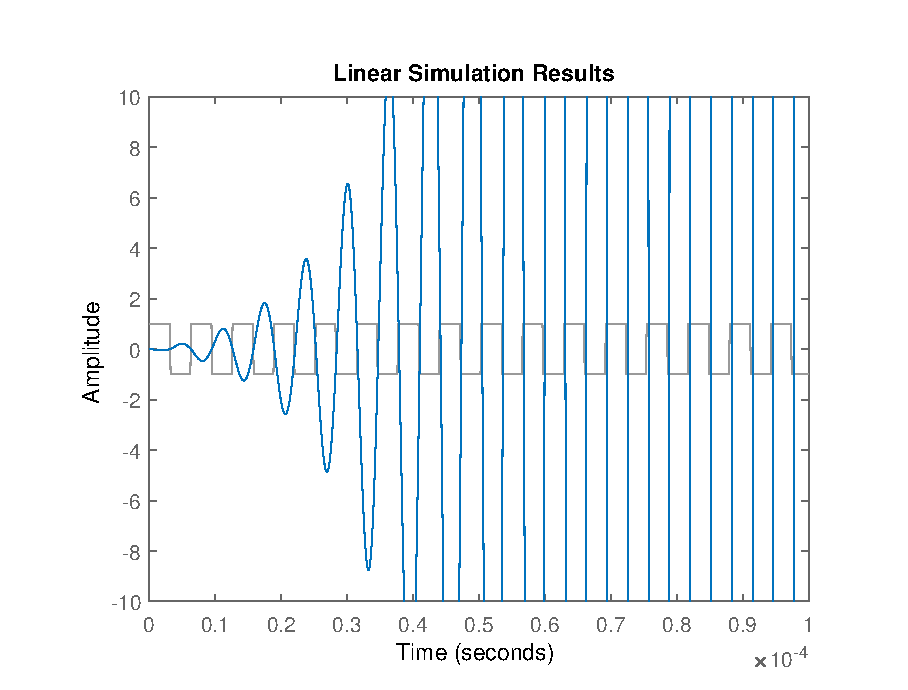
\includegraphics[width=\textwidth]{img/Simulation.eps}
    \caption{Linear simulation of transfer function with square wave with $f=f_0$ as input}
    \label{fig:my_label}
\end{figure}


\subsubsection{Feedback Transfer function plots}

\begin{figure}
    \centering
    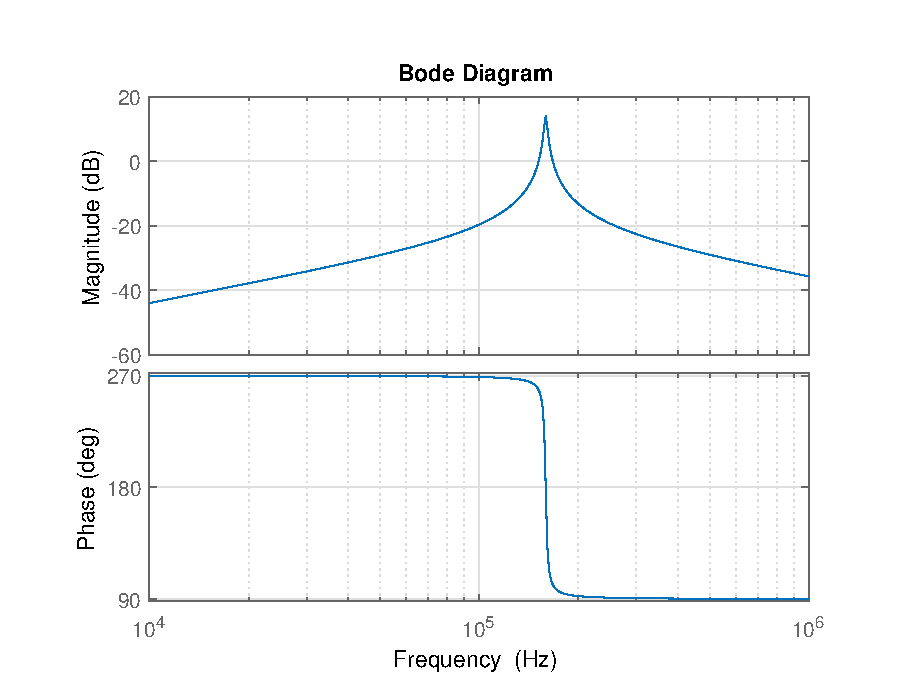
\includegraphics[width=\textwidth]{img/FeedbackBode.eps}
    \caption{Bode plot of the transfer function for the feedback current}
    \label{fig:my_label}
\end{figure}

\begin{figure}
    \centering
    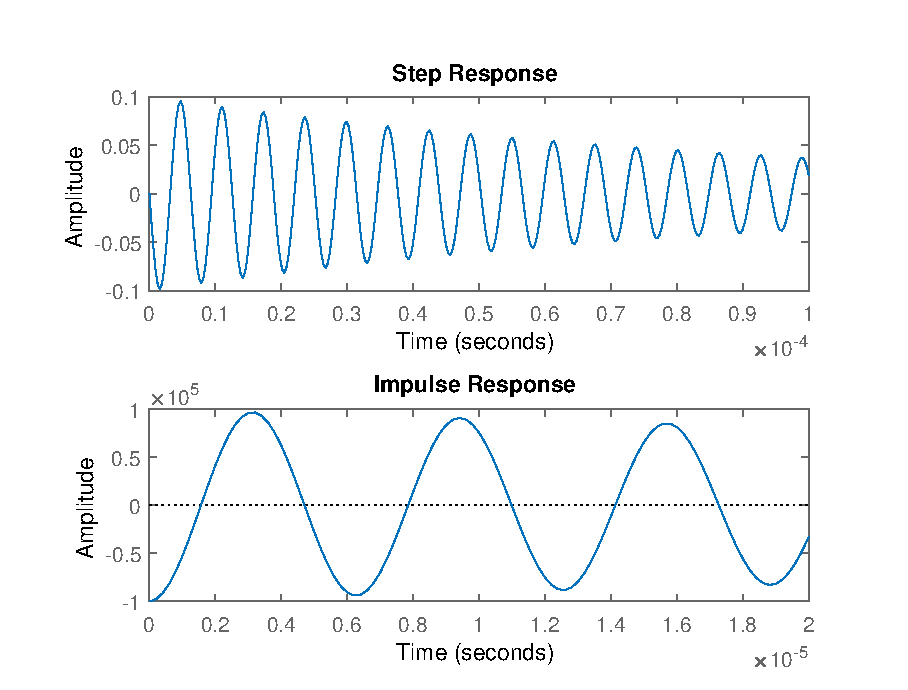
\includegraphics[width=\textwidth]{img/FeedbackResponse.eps}
    \caption{Step and impulse response of transfer function for the feedback current}
    \label{fig:my_label}
\end{figure}

\subsection{Magnitude analysis}
By taking the magnitudes for each variable listed in \cref{tab:mod_params} and inserting them into the different terms in the transfer function $H(s)$ we can see wich terms influence the result and wich terms are insignificant.

\subsection{Arc}
The arc is modeled as a conductance.
\begin{equation} \label{eq:g1}
    G_1 = G_{min} + [ 1 - exp(-\frac{i_{G1}^2}{I_0^2})] \frac{u_s i_{G1}}{E_0^2} + [exp(-\frac{i_{G1}^2}{I_0^2})] \frac{i_{G1}^2}{P_0} - \theta \frac{d G_1}{dt}
\end{equation}

\begin{equation}
    \theta = \theta_0 + \theta_1 exp(-\alpha |i|)
\end{equation}

\begin{table}[h]
    \centering
    \begin{tabular}{c|c|c|c}
         & Comment &  &\\ \hline
        $\theta$  & Arc dampening factor &  &\\
        $G_{min}$ & Least possible conductance &  &\\
        $I_o$     & Limit between large and small current &  &\\
        $E_0$     & Constant, steasy state arc voltage &  &\\
        $P_0$     & Constant power loss from arc &  & \\
        $i_{G1}$  & Current flowing in arc      &  & \\
        $u_s$     & Voltage over arc            &  &
    \end{tabular}
    \caption{Caption}
    \label{tab:my_label}
\end{table}
